\chapter{Data Generation and Exploration}
\label{sec:exploration}
\ifpdf
    \graphicspath{{4_data_exploration/figures/PNG/}{4_data_exploration/figures/PDF/}{4_data_exploration/figures/}}
\else
    \graphicspath{{4_data_exploration/figures/EPS/}{4_data_exploration/figures/}}
\fi


Nikhef provided simulated data from three sources that were used to generate the complete KM3NeT dataset - the \textit{K40 noise generator}, \textit{HDF5 hits and events} tables and a \textit{positions} file. This chapter describes the steps taken to combine noise and events data to produce the complete dataset. The chapter then discusses the quality and properties of the complete dataset by means of visual data exploration. 

\section{Noise Generation}
Noise for the dataset was generated using the \textit{k40gen} \footnote{https://gitlab.nikhef.nl/roelaaij/k40gen} package. \textit{k40gen} is a standalone background noise generator developed by Nikhef to generate a random array simulating Potassium-40 decay underwater. An instance of the generator was created with two random seeds - \texttt{21341} and \texttt{1245}. \texttt{7000}, \texttt{700}, \texttt{70}, and \texttt{0} were specified as the rates at which single, double, triple, and quadruple hits were to be generated respectively. Noise hits were generated from \texttt{0} nanoseconds (ns) till \texttt{100000000} ns. The ORCA (Oscillation Research with Cosmics in the Abyss) counting scheme was also provided as a numbering scheme for the photomultiplier (PMT) IDs within the Digital Optical Modules (DOMs). The DAS-5 cluster \footnote{https://www.cs.vu.nl/das5/} was used to install and generate the background noise array, totalling 5GB. The returned array contained information regarding \texttt{time}, \texttt{DOM ID}, \texttt{PMT ID} and \texttt{time-over-threshold} for noise hits.

Additionally, the positions file (\texttt{positions.detx}) contained all the spatial positions corresponding to the noise hits from the \textit{k40gen} array and had to be merged. Spatial positions from \texttt{positions.detx} were identified and mapped to the corresponding noise hits using the following formula:

\begin{equation}
    noise[pos\_idx] = 31 \times (noise[dom\_id] - 1) + noise[pmt\_id])
\end{equation}

Finally, a class label of \texttt{0} was also added for all hits to indicate noise for future classification. 


\section{Event Hits Generation}
Neutrino events data was stored in a HDF5 (Hierarchical Data Format version 5) file \footnote{https://www.hdfgroup.org/solutions/hdf5/} consisting of an event hits table (\texttt{mc\_hits}) and a corresponding event information table (\texttt{mc\_info}). \texttt{mc\_hits} included information pertaining to the DOMs (\texttt{dom\_id}), PMTs (\texttt{pmt\_id}),  positions (\texttt{pos\_x, pos\_y, pos\_z}) and directions (\texttt{dir\_x, dir\_y, dir\_z}) of event hits. It also contained time over threshold (\texttt{tot}) values and the time the hits were registered (\texttt{time}). A class label of \texttt{1} was added to this data to indicate an event hit. Only the \texttt{mc\_hits} table was used for the classification project undertaken in this thesis. 


\section{Data Combination}
Before the background noise and event hits data could be combined, a few preliminary cleanup and validation measures were taken. First, it was noticed that the PMT IDs for event hits were from \texttt{0} till \texttt{6417}. This indicated that it followed a global numbering scheme, while PMT IDs for noise hits had been generated using the ORCA numbering scheme. To enforce uniformity, PMT IDs for event hits were set from \texttt{1} till \texttt{31}: 

\begin{equation}
    pmt\ id = pmt\ id - 31 \times (dom\ id - 1)
\end{equation}

Next, \texttt{time} for some noise hits were negative, so these data points were deemed invalid and deleted from the dataset. As both events and noise data were simulated, it was important to ensure that the \texttt{time} values associated with event hits were not biased. To check for such a bias, the mean time of occurrence for all event hits was calculated and plotted for any evidence of hits clusters. Based on the evenly distributed scatter of points in Figure \ref{fig:bias_verification}, it was concluded that there were no biases in the data. Noise and event hits were merged to form the complete KM3NeT dataset after negative time was deleted, PMT IDs were adjusted and data validity was confirmed.

\begin{figure}[ht!]
    \centering
    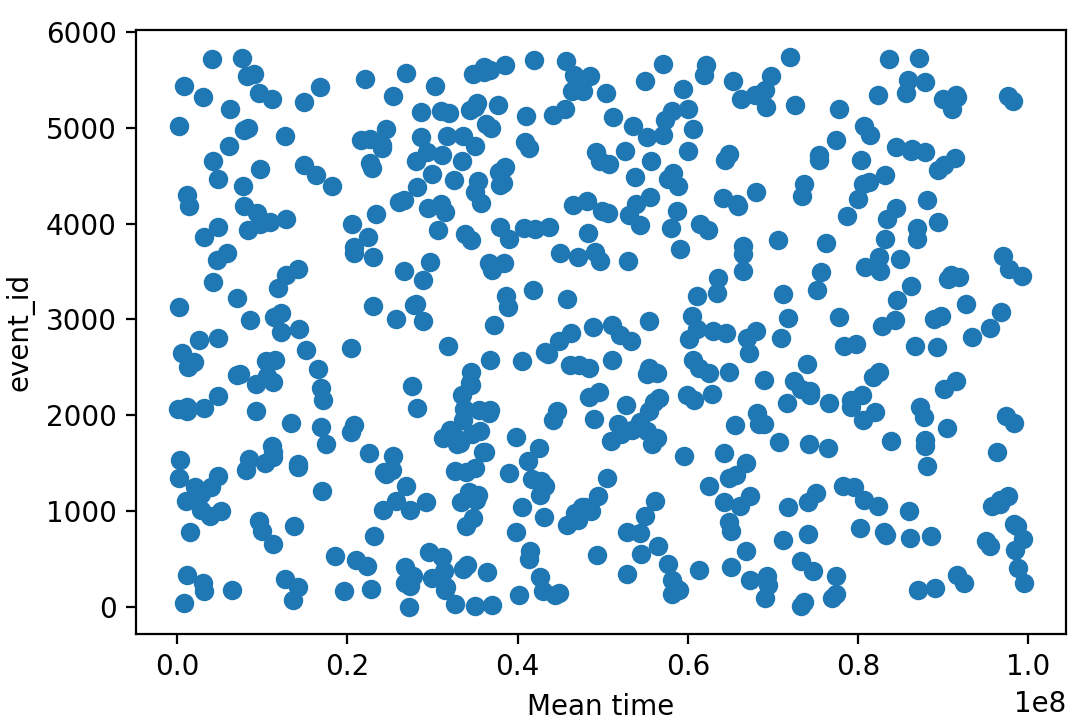
\includegraphics[width=0.7\textwidth, height=7cm]{bias_verification.png}
    \caption{Scatter Plot of Mean Time for All Event Hits}
    \label{fig:bias_verification}
\end{figure}



\section{Key Attributes}
The KM3NeT detector records and sends data in chunks (timeslices) for processing at the offshore facility \cite{km3net_2017}. The thesis's main aim was to train a network that would classify timeslices into those that contained only noise and those that contained event hits amidst noise. Therefore, the dataset was sequentially binned into groups of 15000 ns and assigned a number for identification. For example, timeslice \texttt{0} contained all hits that occurred between 0 ns and 15000 ns. 15000 ns was used for binning as neutrino events typically occur between 100 ns and 15000 ns \cite{km3net_2017}. Selecting a value on the higher end of the range allowed for fewer groups to be created and by extension, faster processing. The binning resulted in a total of 6759 groups. The complete dataset was found to be 4GB in size, with 45,820,220 rows and 12 attributes, summarised in Table \ref{tab:attributes}.

\begin{table} [ht!]
    \begin{tabular}{l l}
    \hline
        \textbf{Attribute} & \textbf{Description} \\
    \hline
       \texttt{dom\_id} & [Unique ID for sensor module.] \\
       \texttt{pmt\_id} & [Unique ID for photomultiplier (PMT) tubes within DOMs.] \\
       \texttt{pos\_x, pos\_y, pos\_z}  & [Spatial coordinates (in meters) of hit within the detector.] \\
       \texttt{dir\_x, dir\_y, dir\_z} & [Direction of PMT tubes within DOMs to look for \\
                                       & Cherenkov Light.] \\
       \texttt{tot}   & [Time-over-threshold (ToT) indicates the amount of light \\
                      & transformed to charge which is interpreted as the length \\
                      & of the square wave pulse over a given threshold \cite{karas_2019}.] \\
       \texttt{time}  & [Time at which the hit was recorded.]\\
       \texttt{label} & [0 or 1 class label indicating whether hit is from noise or \\
                      & event respectively.]\\
       \texttt{group} & [Timeslice numbers starting from 0 for the purpose \\
                      & of identification.] \\
    \hline
    \end{tabular}
    \caption{KM3NeT Data Attributes and Description}
    \label{tab:attributes}
\end{table}


Domain knowledge from Nikhef indicated \texttt{dom\_id, pmt\_id} and direction of PMT tubes (\texttt{dir\_x, dir\_y, dir\_z}) to be metadata that could be ignored. Additionally, work by Karas (2019) identified time-over-threshold (\texttt{tot}) to be insignificant to the classification problem \cite{karas_2019}. The remaining attributes - spatial coordinates (\texttt{pos\_x, pos\_y, pos\_z}), \texttt{time}, \texttt{label} and timeslices (\texttt{group}) were identified as key variables for the remainder of the classification project. 


\section{Visual Analysis}

\begin{figure}[ht!]
    \centering
    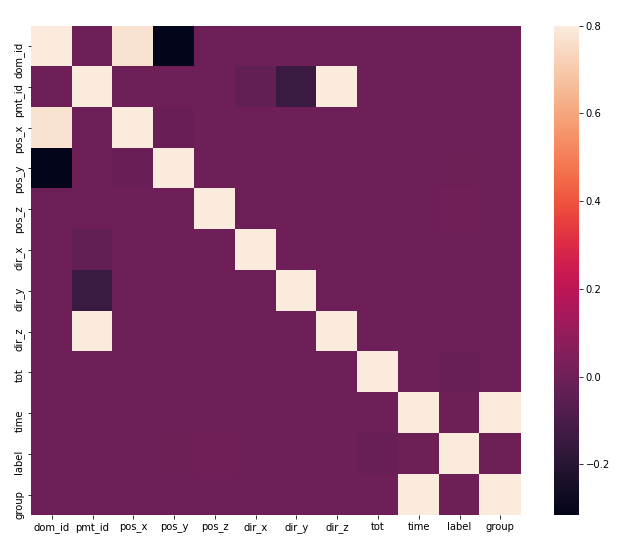
\includegraphics[width=0.7\linewidth, height=7cm]{correlations.png}
    \caption{Correlation Heatmap Between Variables}
    \label{fig:corr}
\end{figure}

Python libraries were used to explore the quality of the dataset and gain further insight on the key variables and the relationships that may exist between them. The dataset was found to have no missing values or outliers. All hits occurred between \texttt{0} ns till \texttt{101591357} ns. The dataset showed severe imbalance between event hits and noise as, for every 1 event hit, there were 93 noise hits. Finally, the correlation heatmap in Figure \ref{fig:corr} indicated that the key variables had no relevant relationship with each other. Significant variables were further examined to identify existence of useful properties.


\subsubsection*{Timeslices (\texttt{group}):} 
Timeslice \texttt{0} was found to have the highest number of hits (12,454), all of which were noise. Timeslice \texttt{615} contained the highest number of event hits (around 8500) with the lowest noise-to-event hits ratio of 4:1. Figure \ref{fig:points_per_group} shows the distribution of number of points per timeslice. Timeslice \texttt{0} had the highest occurrence of hits while some timeslices contained very few hits. These timeslices were edge cases and were ignored for the rest of the project. However, majority of the other timeslices contained between 6000 to 8000 hits, providing a more or less consistent sample for the training.

\begin{figure}[ht!]
    \centering
    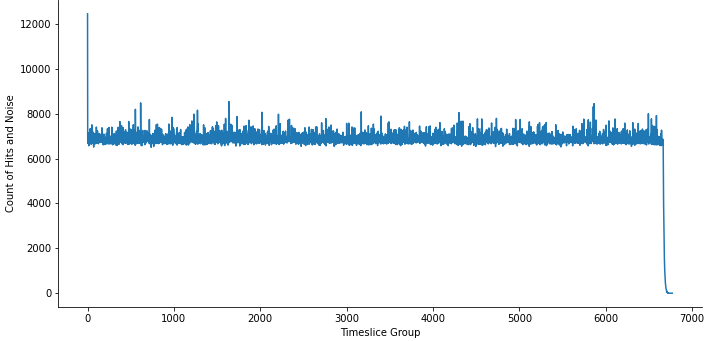
\includegraphics[width=0.7\linewidth, height=5cm,keepaspectratio]{points_per_group.png}
    \caption{Count of Total Points per Timeslice}
    \label{fig:points_per_group}
\end{figure}

In accordance with the classification task, timeslices were separated into those that contained only noise and those that contained both event hits and noise. First, class imbalance between event hits and noise within timeslices were visually examined. Figure \ref{fig:hits_by_group} shows that most timeslices with both events and noise had between 0 to 250 event hits. On the other hand, Figure \ref{fig:noise_by_group} shows noise timeslices had around 7000 points on average. The outliers in this Figure (\ref{fig:noise_by_group}) demonstrate a timeslice that had a significantly large number of noise hits and timeslices towards the end that had comparatively fewer noise hits. These anomalies could be attributed to the nature of the \textit{k40gen} random noise generator. Figure \ref{fig:kde_hits_by_group} and Figure \ref{fig:kde_noise_by_group} use kernel density estimation (KDE) to produce a continuous density estimate using a Gaussian Kernel and provides an alternate visualisation of the severe class imbalance by highlighting the densest regions \cite{waskom2020seaborn}.


\begin{figure}[ht!]   
\centering
\subfloat[Count of Event Hits For Timeslices with Both Noise and Events]{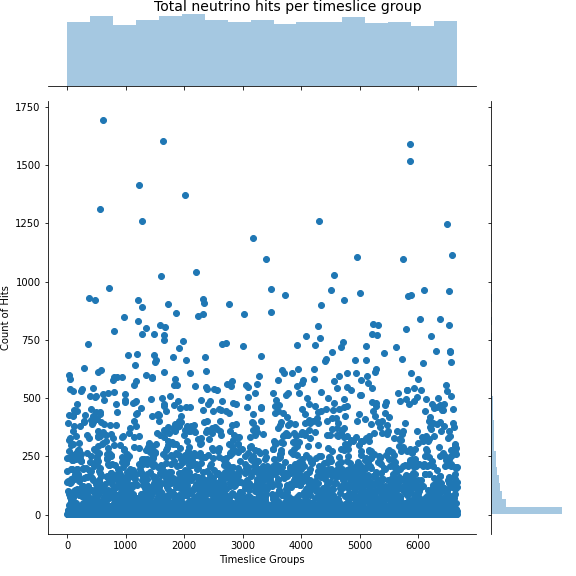
\includegraphics[trim={0 0 0 0.51cm}, clip, width=0.5\textwidth, keepaspectratio]{hits_by_group.png}\label{fig:hits_by_group}}
\subfloat[Count of Noise Hits For Timeslices with Only Noise]{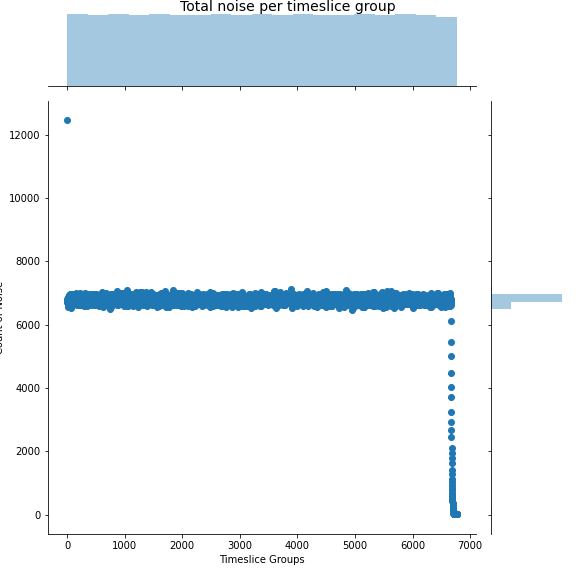
\includegraphics[width=0.5\textwidth,
height=7.4cm,keepaspectratio]{noise_by_group.png}\label{fig:noise_by_group}}

\subfloat[Kernel Density Estimation for Only Event Hits]{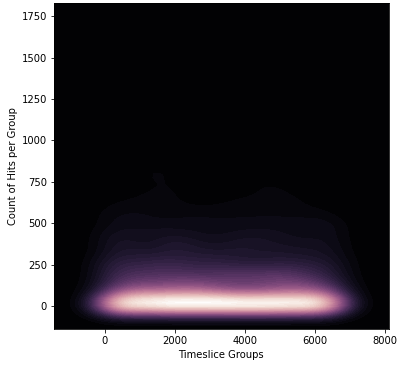
\includegraphics[trim={0 0 0 0.51cm}, clip, width=0.5\textwidth, keepaspectratio]{kde_hits_per_group}\label{fig:kde_hits_by_group}}
\subfloat[Kernel Density Estimation for Only Noise Hits]{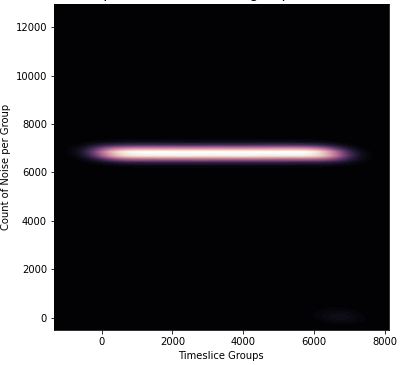
\includegraphics[width=0.5\textwidth,
height=7.4cm,keepaspectratio]{kde_noise_per_group}\label{fig:kde_noise_by_group}}
\caption{Comparing Count of Hits and Noise Between Timeslices}
\label{fig:kde_comparing_groups}
\end{figure}

\subsubsection*{3D Spatial Coordinates (\texttt{pos\_x, pos\_y, pos\_z}):} 
Figure \ref{fig:615_points} uses a "swarm" technique to show distribution of noise and event hits across time for timeslice \texttt{615}, the group with the highest incidence of event hits. The points are non-overlapping and adjusted to better show distribution \cite{waskom2020seaborn}. Orange points indicate that event hits occur in groups coinciding with neutrino events amidst the noise. 

\begin{figure}[ht!]
    \centering
    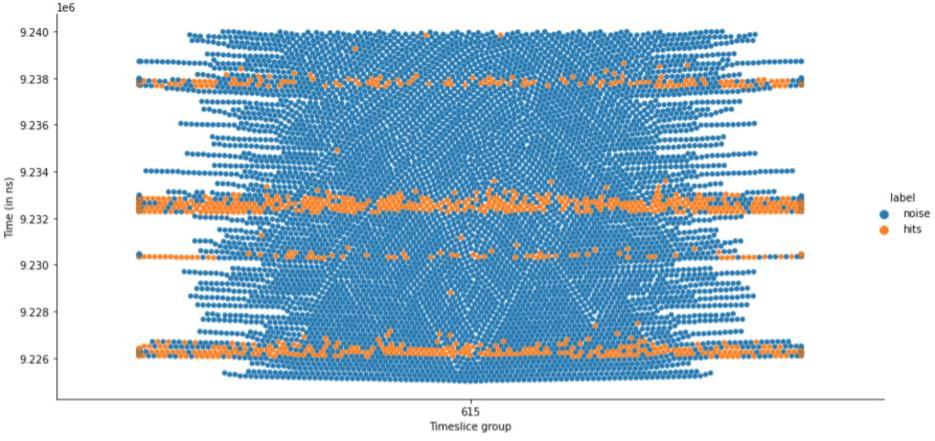
\includegraphics[width=0.7\linewidth,keepaspectratio]{615_point_distribution.jpg}
    \caption{Distribution of Noise and Event Hits in Timeslice 615}
    \label{fig:615_points}
\end{figure}

Bi-variate plots in Figure \ref{fig:x_y_z} show the relationship between the \texttt{x, y, z} points for timeslice \texttt{615}. These 3D coordinates don't give much information or patterns that may indicate presence of event hits, confirming the need for \texttt{time} as part of the dataset.

\begin{figure}[ht!]   
\centering
\subfloat[Scatter plot for \texttt{pos\_x} against \texttt{pos\_y}]{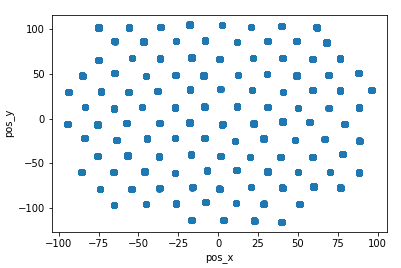
\includegraphics[width=0.33\textwidth,height=5cm]{x_y.png}\label{fig:xy}}
\subfloat[Scatter plot for \texttt{pos\_x} against \texttt{pos\_z}]{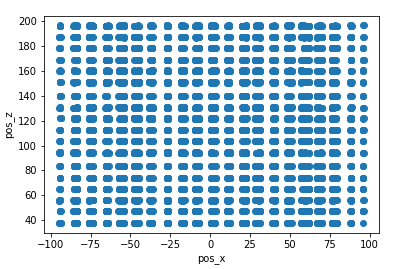
\includegraphics[width=0.33\textwidth,
height=5cm]{x_z.png}\label{fig:xz}}
\subfloat[\texttt{pos\_y} against \texttt{pos\_z}]{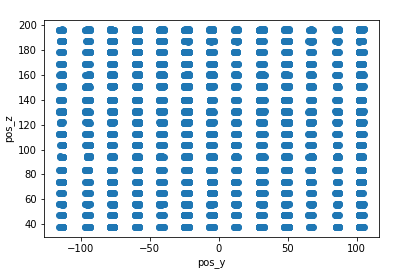
\includegraphics[width=0.33\textwidth,
height=5cm]{y_z.png}\label{fig:yz}}
\caption[]{Bi-variate Plots Showing Relationship Between 3D Coordinates}
\label{fig:x_y_z}
\end{figure}

Figure \ref{fig:fig:0_615} shows an enhanced 3D render of timeslice \texttt{615} generated using MeshLab \footnote{https://www.meshlab.net/}. The timeslice is first visualised as \texttt{x}, \texttt{y} and \texttt{time}, then \texttt{x, z} and  \texttt{time} and finally \texttt{y, z,} and \texttt{time}.  The three representations show no relevant differences between each other. However, visual enhancements via MeshLab allow for event clusters to stand out, as indicated by the bright clusters of points.

\begin{figure}[ht!]   
\centering
\subfloat[3D Plot of \texttt{x, y, time}]{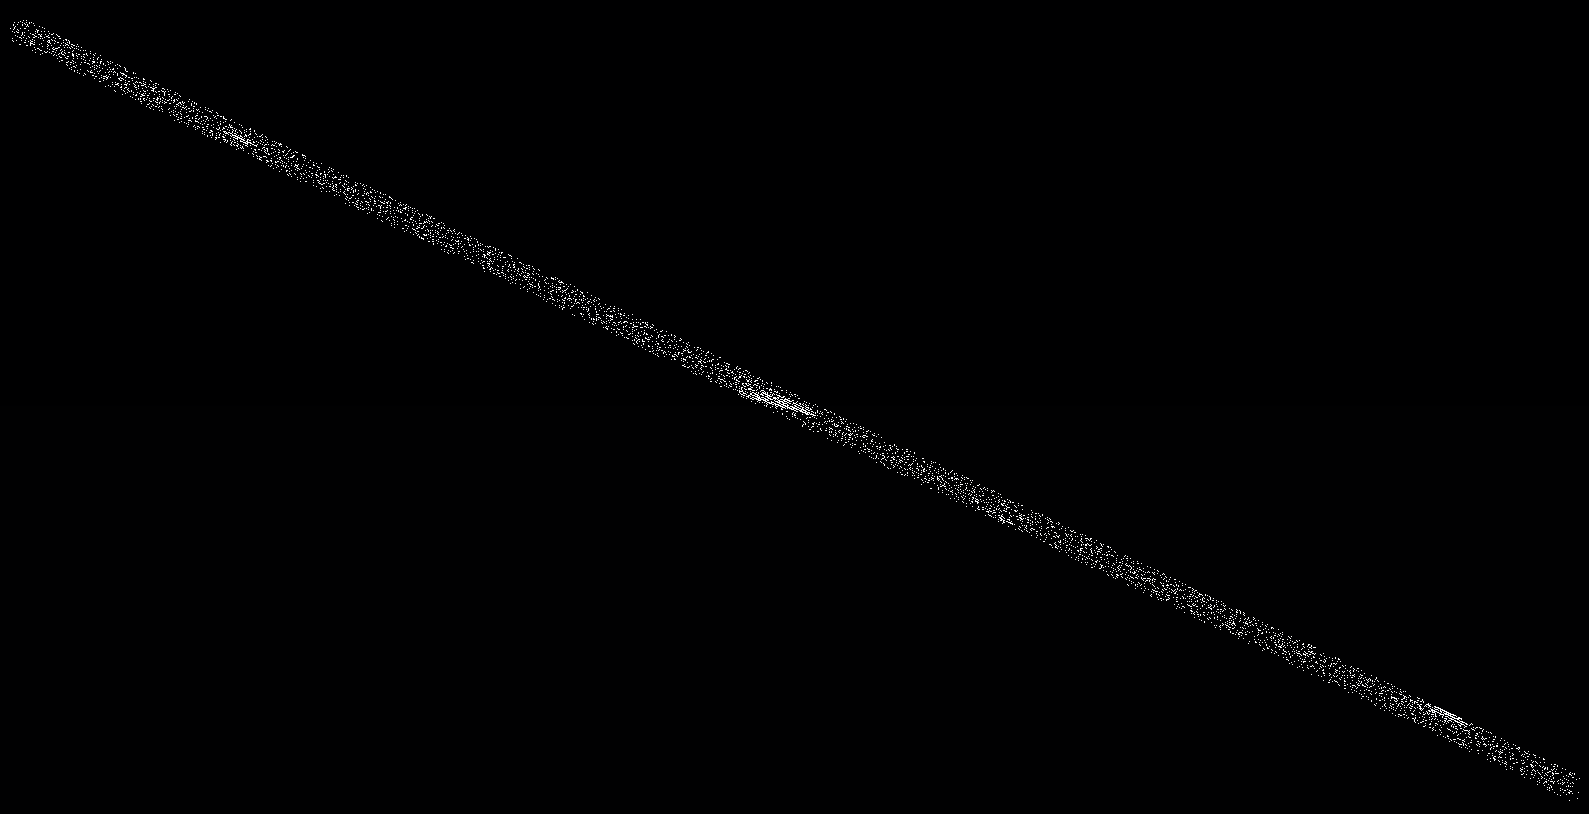
\includegraphics[width=0.32\textwidth,height=5cm]{xyt.png}\label{fig:xyt}}
\hspace{0.01cm}
\subfloat[3D Plot of \texttt{x, z, time}]{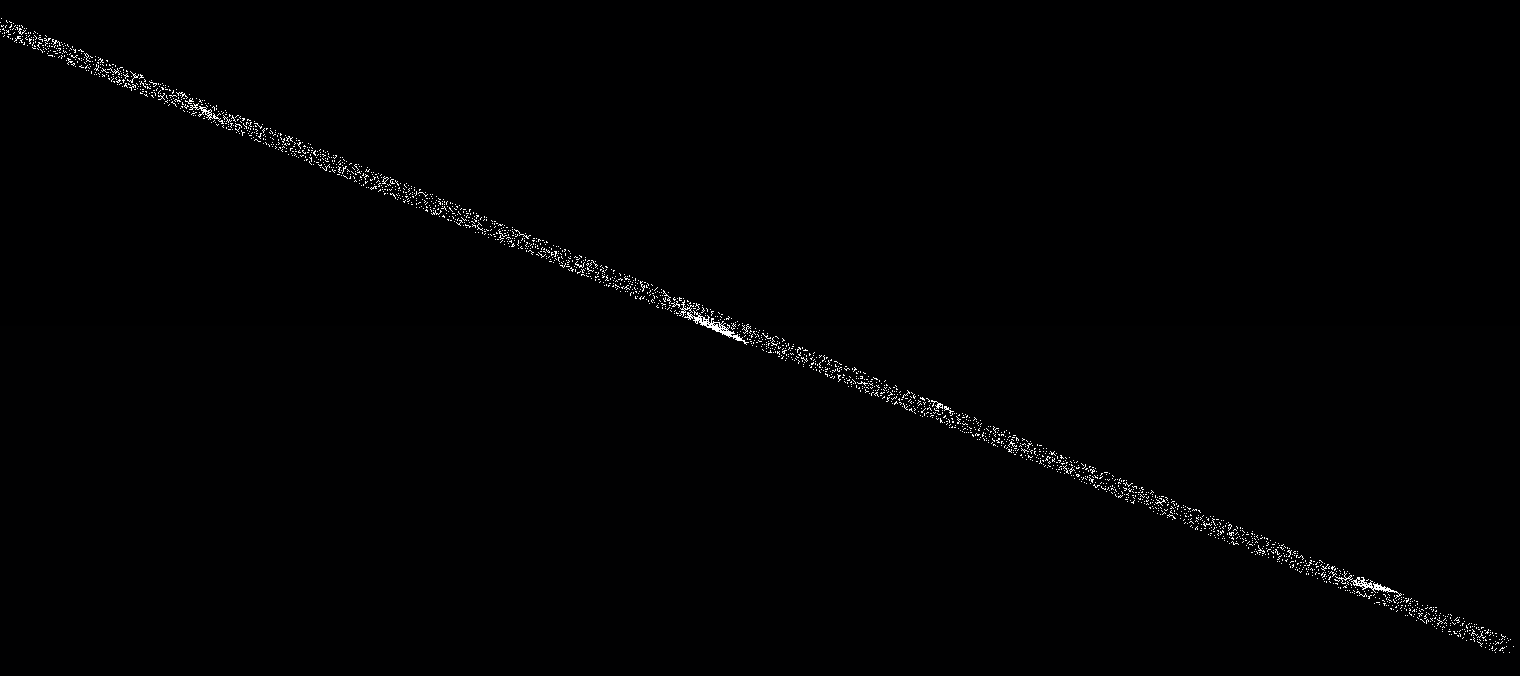
\includegraphics[width=0.32\textwidth,height=5cm]{xzt.png}\label{fig:xzt}}
\hspace{0.01cm}
\subfloat[3D Plot of \texttt{y, z, time}]{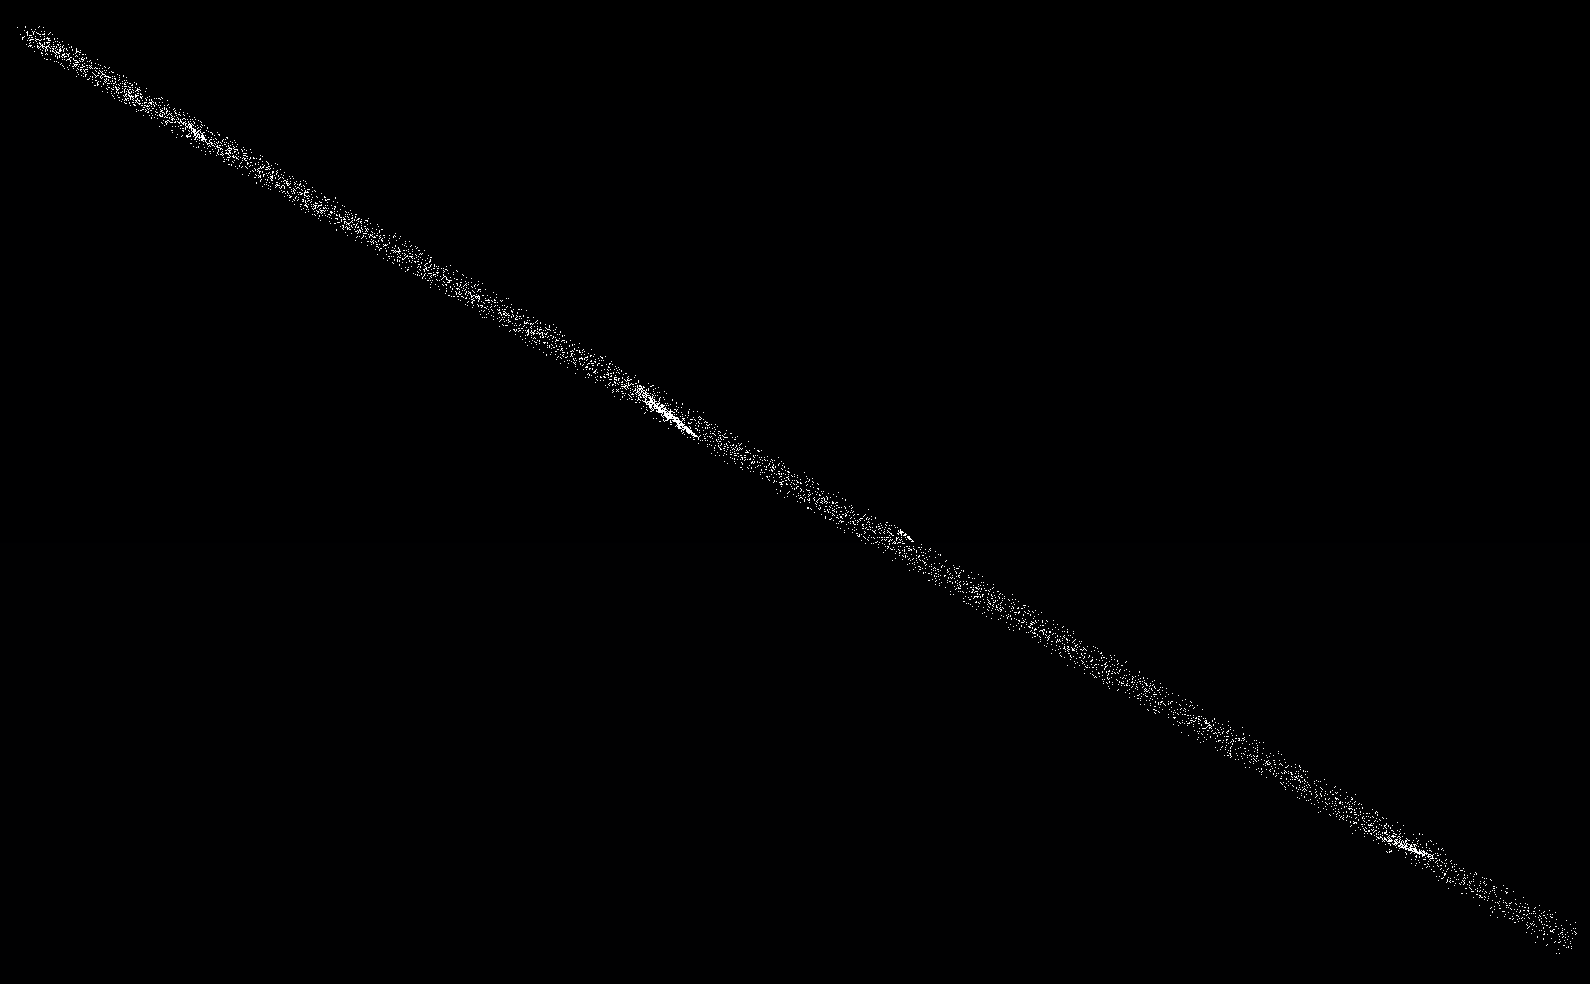
\includegraphics[width=0.32\textwidth,height=5cm]{yzt.png}\label{fig:yzt}}
\caption[]{3D Plots Showing Combinations of \texttt{x, y, z, time} for Timeslice 615}
\label{fig:fig:0_615}
\end{figure}

\subsection*{Time (\texttt{time})}
Time plays a significant role in the identification of neutrino hits amidst noise. A swarm plot of \texttt{time} against \texttt{label} was plotted for two events timeslices to note the relation between time and type of hit \cite{eklund2012beeswarm}. Figure \ref{fig:time} shows an even distribution of noise hits across time, while event hits again form localised clusters.

\begin{figure}[ht!]   
\centering
\subfloat[\texttt{time} and \texttt{label} for Timeslice 615]{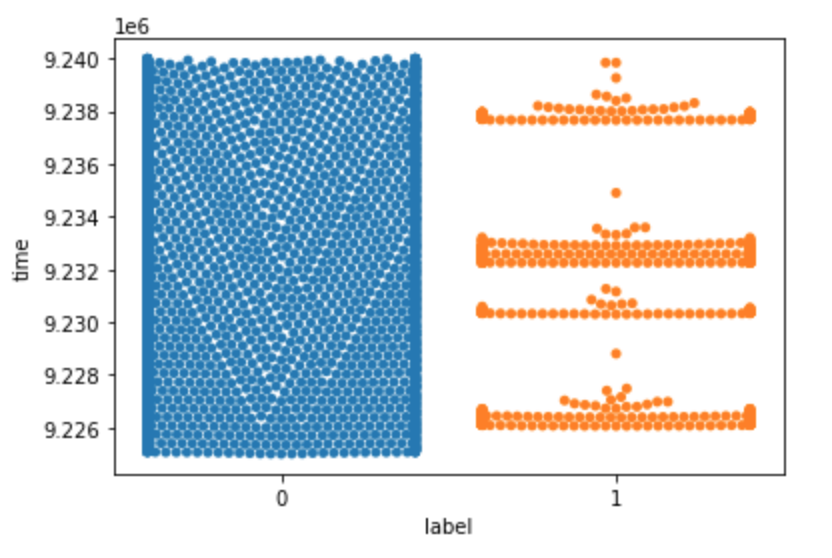
\includegraphics[width=0.5\textwidth,height=10cm, keepaspectratio]{label_time_615.png}}
\subfloat[\texttt{time} and \texttt{label} for Timeslice \texttt{1637}]{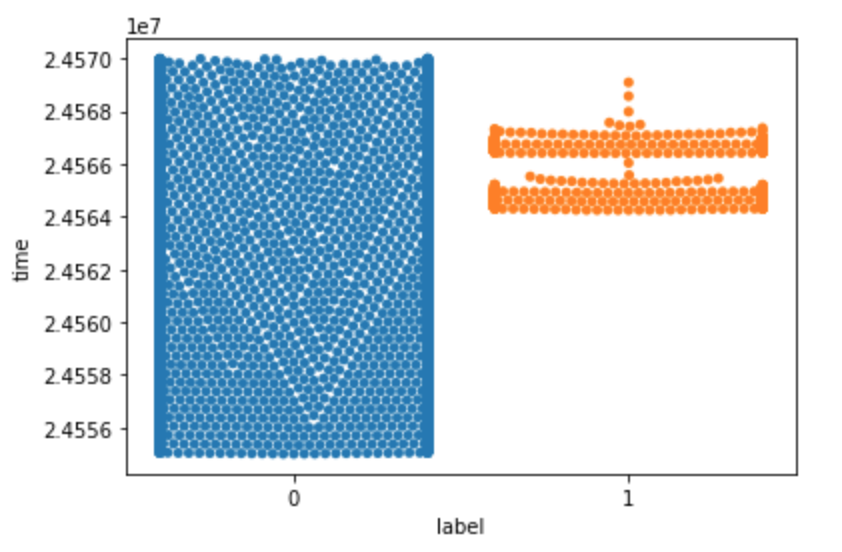
\includegraphics[width=0.5\textwidth,height=10cm, keepaspectratio]{time_label_1637.png}}
\caption[]{Swarm Plots Showing Relationship Between Time and Hit Labels}
\label{fig:time}
\end{figure}

Based on the combined results from plots of spatial positions, \texttt{time} and \texttt{label}, it was evident that a combination of these attributes would be required to obtain sufficient information on event hits. Further, the dataset had unrelated variables, lacked significant patterns, and had a high density of points. It would be very likely that the network would not be able to learn anything significant. Therefore, feature engineering may be required to add new information to the dataset before training could occur. 

\let\cleardoublepage\clearpage
